\chapterimage{chapter_head_2.pdf} % Chapter heading image

\chapter{\textcolor{blue}{Fundamentos de musicalidade}}

\begin{definition}[Musicalidade:] 
\index{Musicalidade}
\label{def:Musicalidade}
O Dicionário Online de Português define musicalidade como \cite{diciomusicalidade}:
\begin{itemize}
\item Particularidade, característica ou estado do que é musical.
\item Tendência natural, \textbf{sensibilidade} ou talento para criar ou tocar música.
\item \textbf{Sensibilidade} para contemplar música; \textbf{conhecimento} sobre música.
\item A \textbf{demonstração do talento} musical de uma pessoa.
\end{itemize}
\end{definition}



%% Informação mutua vs Correlação
%% Exemplo dançar em coerencia com a música
%% Eurythmics - Sweet Dreams (Are Made Of This) (Official Video)

%%%%%%%%%%%%%%%%%%%%%%%%%%%%%%%%%%%%%%%%%%%%%%%%%%%%%%%%%%%%%%%%%%%%%%%%%%%%%%%%
%%%%%%%%%%%%%%%%%%%%%%%%%%%%%%%%%%%%%%%%%%%%%%%%%%%%%%%%%%%%%%%%%%%%%%%%%%%%%%%%
\section{Musicalidade, sentir ou entender a música?}
Seguindo a Definição \ref{def:Musicalidade}, podemos inferir como entender a musicalidade na dança.
\begin{definition}[Musicalidade na dança:] 
\index{Musicalidade}
\label{def:MusicalidadeNaDanca}
Esta acontece, quando o dançarino tem um estado de ``sensibilidade'' ou ``conhecimento'' para contemplar ou entender a música,
e assim quando este dança, ``demostrar'' uma coerência entre a música e o que está dançando.
\end{definition}

Porem temos um choque de paradigmas, na definição, para atingir um mesmo objetivo que é ser musical.
Podemos \textbf{sentir} ou \textbf{conhecer}; o que é equivalente a dizer que:
\begin{itemize} 
\item podemos saber, por intuição sem entender porquê, ou
\item podemos saber, entendendo mediante o conhecimento adquirido pelo raciocínio e o estudo.\\
\end{itemize}



Neste sentido, para adquirir esta coerência com a música, 
muitos professores indicam que o dançarino deve ``escutar e sentir a música'';
nesse aspecto, argumento que a frase é metaforicamente correta e coincide em parte com 
a Definição \ref{def:Musicalidade} e a Definição \ref{def:MusicalidadeNaDanca};
porem, pedagogicamente  é pouco favorável para o estudante.
Assim, eu ressaltaria que a musicalidade a nível de ensino se adquire,
estudando e entendendo a música e não só sentindo-a.
 
Para fundamentar minha argumentação, acredito interessante expor o seguinte exemplo: 
\begin{example}
Imaginemos que conhecemos ao matemático ``Srinivasa Aiyangar Ramanujan'';
um prodígio matemático autodidata \cite[pp. 1]{kanigel2016man}, indiano, que 
realizou muitas contribuições à matemática.
E mostramos a ele um problema matemático, como por exemplo uma equação,
e  lhe pedimos a resposta ou solução. 
Então Srinivasa, muito amavelmente, 
observaria um instante o problema e nos daria a solução imediatamente.
Nós surpreendidos pela velocidade e o mínimo esforço na resposta,
perguntaríamos. Como você obteve a resposta? Então ele responderia \cite[pp. 235]{kanigel2016man}: 
%\begin{citando}
%Immediately I heard the problem 
%it was clear that the solution should obviously be a continued fraction; 
%I then thought, Which continued  fraction? And the answer came to my mind.
%\end{citando}
\begin{citando}
No momento em que escutei o problema, 
foi claro pra mim que a resposta devia ser obviamente uma fração continua; 
E então pensei, ¿Qual fração continua? e a resposta chegou a minha mente. 
\end{citando}
\end{example}

A resposta que ele deu, 
é a mesma  que dão as pessoas, quando  dizem que para ter musicalidade ele simplesmente sentiu a música. 
Assim, esta aproximação ao problema é só válida ou eficiente, para pessoas como Srinivasa, 
que talvez tenham uma inspiração divina, 
ou que já nasceram com esse dom ou que por uma longa experiencia de vida, 
tem implementado por ``hardware'', no cérebro, entender a música; 
pelo que eles usam a palavra sentir, 
pois conhecem a resposta, porem não sabem como sabem. 

Isto também pode acontecer com pessoas que observaram muito tempo um ``problema'' ou escutaram muito uma ``canção'', 
e um dia conseguiram ``sentir'' a resposta. Na minha opinião não todos nascemos, 
com esse componente, implementado em nosso cérebro, para entender  a música; 
e não podemos nos dar o luxo de escutar uma canção indefinidamente ate sentir algo; 
o mais eficiente seria estudar música, 
e entender esta baseando-nos em nossa teoria e cruzando esta informação com o que escutamos, 
os padrões observados, a melodia, o ritmo, etc. 
Assim, nos podemos criar por ``software'' o que não temos implementado por ``hardware'', 
derrubando o mito de ``sentir'' a música e passar a ``entender'' ela.


%%%%%%%%%%%%%%%%%%%%%%%%%%%%%%%%%%%%%%%%%%%%%%%%%%%%%%%%%%%%%%%%%%%%%%%%%%%%%%%%
\section{\textcolor{blue}{Interpretação corporal da música}}

Figura \ref{fig:interpretacion-corporal}.

interpretação corporal se divide em:
\begin{itemize}
\item Consciência corporal
\item Controle corporal
\item Dissociação corporal
\item Expressão corporal
\end{itemize}
mais informação no capítulo \ref{fig:bodyrelations}.

\begin{figure}[!h]
  \centering
    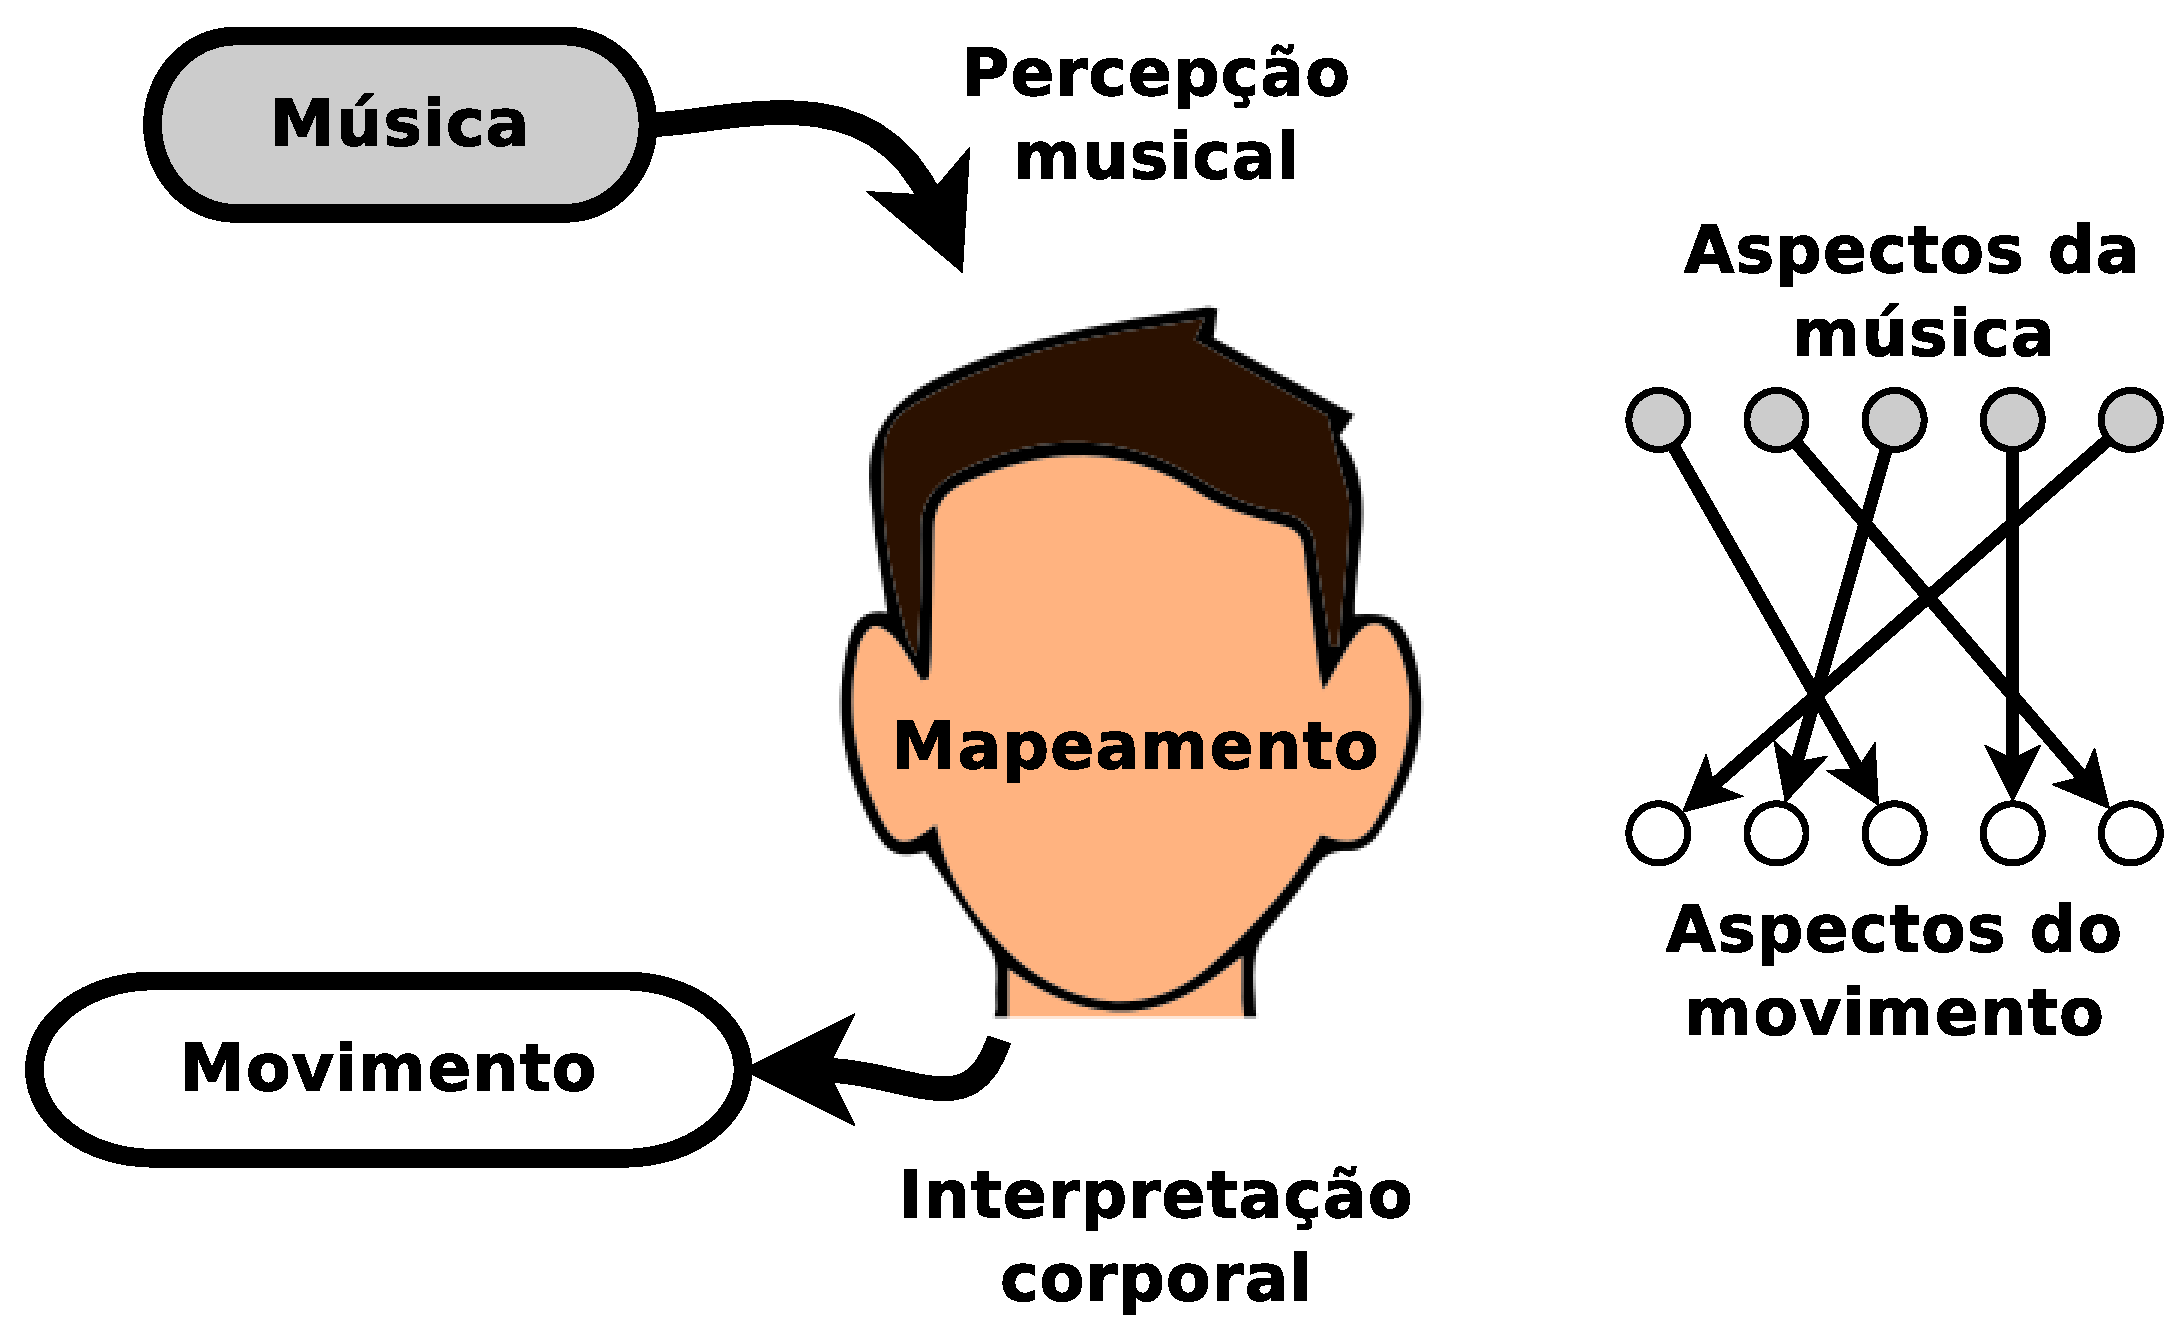
\includegraphics[width=0.5\textwidth]{chapters/cap-musicalidade/interpretacion-corporal.eps}
\caption{Interpretação corporal da música.}
\label{fig:interpretacion-corporal}
\end{figure}



%%%%%%%%%%%%%%%%%%%%%%%%%%%%%%%%%%%%%%%%%%%%%%%%%%%%%%%%%%%%%%%%%%%%%%%%%%%%%%%%
%%%%%%%%%%%%%%%%%%%%%%%%%%%%%%%%%%%%%%%%%%%%%%%%%%%%%%%%%%%%%%%%%%%%%%%%%%%%%%%%
\section{\textcolor{blue}{Contagens dos passos para o ensino}}
Antes de iniciar esta seção é importante mencionar uma
problemática que é vista com muita frequência nas escolas de dança; 
esta é gerada devido a que: A forma em que os tempos são contados 
na música, é
diferente à realizada entre profissionais da música e da dança. 
Sendo que a contagem dos profissionais da música segue a \hyperref[def:Metrica]{\textbf{métrica}} indicada na partitura,
e no caso de profissionais da dança segue geralmente um enfoque 
particular a cada escola de dança, visando só em muitos casos o fácil entendimento do aluno da
execução do movimento programado para essa aula, e não uma rigorosidade teórica no uso de termos e 
expressões musicais.




\subsection{Contagem de 3 passos em 2 tempos}
Esta diferença na forma de perceber o inicio e o final do ciclo de repetição,
vista na Seção \ref{sec:percepcaoouvinte}, 
leva a um problema quando se quer ser rigoroso na forma de contar os tempos nos compassos; 
por exemplo, na Tabela \ref{tab:ritmo1} 
podemos ver 4 formas distintas, que podem adotar as pessoas, 
para contar os tempos nos compassos indicando a distribuição de tempos, 
onde ``$T$'' representa um tempo do compasso.
\begin{table}[ht]
  \centering
  \begin{tabular}    {c|ccc|c}
    \hline
    Tipos de contagem       & $T/2$ & $T/2$   & $T$ (Forte) & Recomendável?\\
    \hline
    Contagem 1: & tchic  & tchic  & tum   & Sim\\
    Contagem 2: & 2     & e     & 1     & Sim\\ \hline
    Contagem 3: & Con   & tra  & Tempo & Não\\
    Contagem 4: & 1     & e     & 2     & Não\\  \hline
    Contagem 5: & 1     & 2     & 3     & Depende\\ \hline
    \hline
  \end{tabular}
  \caption{Tipos de contagem na samba de gafieira.}
\label{tab:ritmo1}
\end{table}

As formas de contagem que recomendo são:
\begin{itemize}
\item \textbf{A contagem 1}, 
devido que a principio, pode ser usada sem aprofundar demasiado 
na notação musical, de modo que só precisa ser explicado que a duração de um 
``tum'' é o dobro que um ``tchic'', e anexar que tipicamente veremos que o ``tum''
acontece no tempo 1 do compasso; 
%de modo que outra contagem valida seria ``tum tchic tchic''; 
porem, a contagem 1 não está restrita ao uso destas silabas (``tchic'' e ``tum''), 
em geral esta contagem representa a quase qualquer padrão de repetição
que use duas silabas diferentes, como por exemplo os padrões: ``ta-ta kum'', ``tic-tic kum'', etc. 
Este tipo de contagem já é muito usada na pratica e na literatura, pois 
podemos achar variantes como ``quick-quick slow'' (rápido-rápido lento no idioma inglês)
ou ``tic-tic tum'' seguindo a notação usada por Perna no seu livro sobre samba de gafieira \cite[pp. 146]{perna2002samba}.
\item \textbf{A contagem 2}, segue a notação de tempos na partitura, este tipo de
contagem é coerente com a musica, porem precisa de uma major explicação, 
para pessoas não iniciadas na musica e a dança. Porem, isto não quer dizer que seu
entendimento seja complexo, e sim que precisa um investimento em horas de aula
um pouco major que a contagem 1.
Mesmo assim, devemos ter cuidado pois pode-se dar o caso que a partitura não tenha compassos binários 
e sim quaternários, com contagens ``2 e 3'' ``4 e 1'', 
criando este tipo de contagem mais caminhos onde podemos perder coerência com a contagem na partitura.\\
\end{itemize}


Entre as contagens que não recomendo estão:
\begin{itemize}
\item \textbf{A contagem 3} (``con-tra tempo''), 
devido a que o uso deste padrão pode confundir às pessoas que desconhecem 
a definição formal do termo contratempo \cite[pp. 16]{mascarenhascurso} \cite[pp. 36]{azevedocompor}, 
e levar a confusão de achar que um contratempo é só uma distribuição de 3 tempos, 
sendo um o dobro dos outros dois, em termos de tempos execução.
\item \textbf{A contagem 4} é não recomendada, devido a que como é visto nas Figuras 
\ref{fig:abc-caquarela} e \ref{fig:abc-contratempo1}, musicalmente a contagem estaria invertida,
dado que tipicamente o ``tum'' se execute no tempo 1.\\
\end{itemize}

Finalmente, a contagem que precisa um cuidado especial:
\begin{itemize}

\item \textbf{A contagem 5} precisa ser bem explicada, 
devido a que não segue a notação musical; 
porem, seu uso é didático e pode ser resgatado,
se fazemos em todo instante uma aclaração, 
que se trata de \hyperref[sec:TemposCoreograficos]{\textbf{tempos coreográficos}}.
Assim, ficara claro para o estudante, que estes não correspondem necessariamente, 
com os tempos musicais que também devem ser ensinados.
Para mais detalhes sobre os tempos coreográficos ver a Seção \ref{sec:TemposCoreograficos}.

%não é recomendada, 
%por motivos similares aos apresentados para a contagem 4. 
%Além do fato que os números atribuídos estão distantes da
%notação verdadeira na partitura, mesmo sim esta houvesse sido escrita num compasso quaternário.
\end{itemize}

\subsection{\textcolor{red}{Contagem de 2 passos em 2 tempos}}


Tabela \ref{tab:ritmoconta2}

\begin{table}[ht]
  \centering
  \begin{tabular}    {c|cc|c}
    \hline
    Tipos de contagem       & $T$ (fraco)  & $T$ (Forte)& Recomendável?\\
    \hline
    Contagem 1: & tum  & TUM  & Sim\\
    Contagem 2: & 2     & 1     & Sim\\
    Contagem 3: & tempo & Tempo & Sim\\ \hline
    Contagem 4: & 1     & 2     & Não\\ \hline
    Contagem 5: & 1     & 3     & Depende\\  \hline
    \hline
  \end{tabular}
  \caption{Tipos de contagem na samba de gafieira.}
\label{tab:ritmoconta2}
\end{table}

Para mais detalhes sobre os tempos coreográficos ver a Seção \ref{sec:TemposCoreograficos}.


%%%%%%%%%%%%%%%%%%%%%%%%%%%%%%%%%%%%%%%%%%%%%%%%%%%%%%%%%%%%%%%%%%%%%%%%%%%%%%%%
%%%%%%%%%%%%%%%%%%%%%%%%%%%%%%%%%%%%%%%%%%%%%%%%%%%%%%%%%%%%%%%%%%%%%%%%%%%%%%%%
\section{\textcolor{blue}{Contagem de tempos correográficos}}
\label{sec:TemposCoreograficos}
\index{Musicalidade!Tempos coreográficos}

falar da possibilidade de contar 123 567 sim se usa um nome diferente a contagem de tempo musical,
exemplo, tempos coreográficos

Ver Figura \ref{fig:contagemtempocoreografico}.
\begin{figure}
    \centering
    \includegraphics[width=\textwidth]{chapters/cap-musicalidade/contagemtempocoreografico.eps}
    \caption{Contando tempos coreograficos.}
    \label{fig:contagemtempocoreografico}
\end{figure}



%%%%%%%%%%%%%%%%%%%%%%%%%%%%%%%%%%%%%%%%%%%%%%%%%%%%%%%%%%%%%%%%%%%%%%%%%%%%%%%%
%%%%%%%%%%%%%%%%%%%%%%%%%%%%%%%%%%%%%%%%%%%%%%%%%%%%%%%%%%%%%%%%%%%%%%%%%%%%%%%%
\section{\textcolor{red}{Procurando um bom ``Timing''}}
\index{Musicalidade!Timing}
Procurando o momento certo

 sincronização 
 %[https://www.infopedia.pt/dicionarios/ingles-portugues/timing]

 sentido de oportunidade 
 %[https://www.infopedia.pt/dicionarios/ingles-portugues/timing]


%%%%%%%%%%%%%%%%%%%%%%%%%%%%%%%%%%%%%%%%%%%%%%%%%%%%%%%%%%%%%%%%%%%%%%%%%%%%%%%%
%%%%%%%%%%%%%%%%%%%%%%%%%%%%%%%%%%%%%%%%%%%%%%%%%%%%%%%%%%%%%%%%%%%%%%%%%%%%%%%%
\section{\textcolor{red}{Dançando no tempo e em contratempo}}
\index{Musicalidade!Dançando no tempo}
\index{Musicalidade!Dançando em contratempo}


Que significa dançar no tempo forte? 
pisar o tum  no tempo forte.

Se percebo que estou pisando no fraco como corrigir?
podemos usar
\begin{itemize}
\item Caminhada em contratempo
\item Fazemos balaços um número impar de vezes.
\end{itemize}


A Figura \ref{fig:tempovscontratempo}.

\begin{figure}[h]
    \centering 
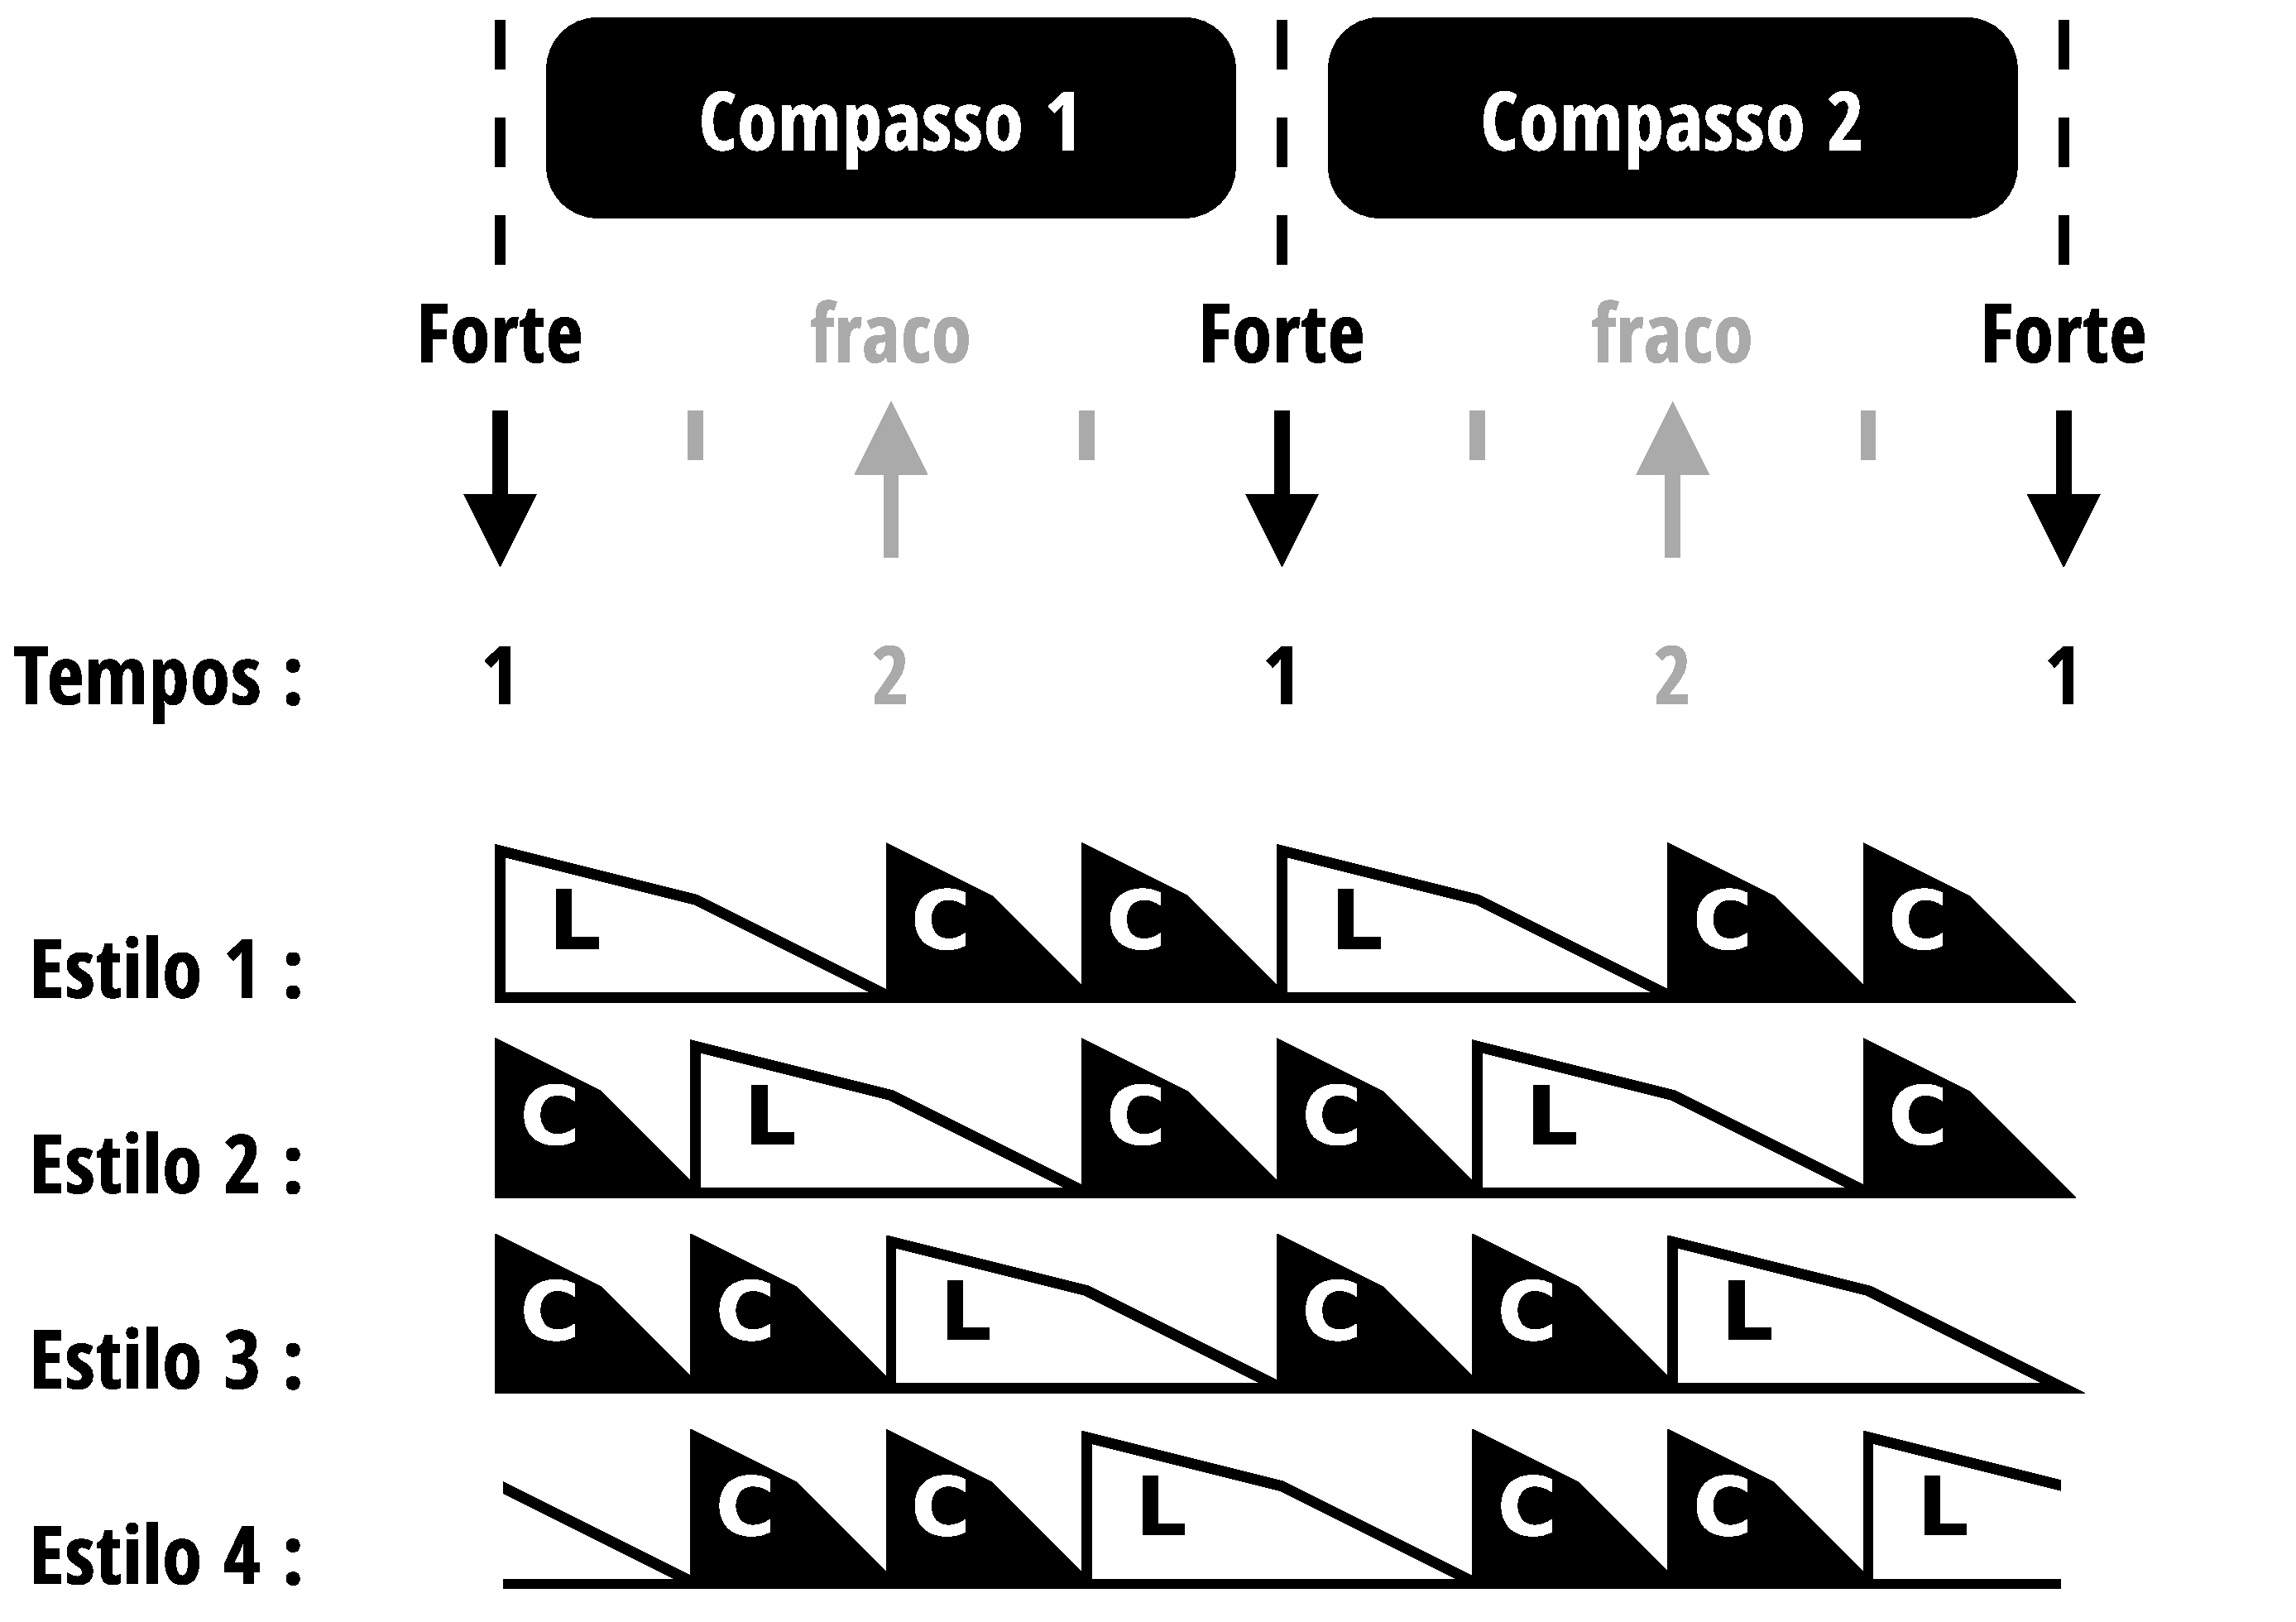
\includegraphics[width=0.9\textwidth]{chapters/cap-musicalidade/bailarcontratempo.eps}
    \caption{Percebendo métrica}\label{fig:tempovscontratempo}
\end{figure}


%%%%%%%%%%%%%%%%%%%%%%%%%%%%%%%%%%%%%%%%%%%%%%%%%%%%%%%%%%%%%%%%%%%%%%%%%%%%%%%%
%%%%%%%%%%%%%%%%%%%%%%%%%%%%%%%%%%%%%%%%%%%%%%%%%%%%%%%%%%%%%%%%%%%%%%%%%%%%%%%%
\section{\textcolor{red}{Percebendo frases musicais}}
\index{Musicalidade!Frase musical}
Porque é importante reconhecer as frases com final conclusivo e suspensivo,
\begin{itemize}
\item Si tentamos dançar no tempo forte, conhecer a existência de ambos tipos de final de frase, 
no ajuda a ter certeza que estamos indo bem com o tempo, e que não somos nos que erramos achando o tempo forte,
e sim, que existe mais de um tipo de final de frase, e que este foi diferente, foi suspensivo.
E não nos deixaremos enganar por finais suspensivos sincopados (que parecem conclusivos),
e estaremos mais seguros de nossa dança.
\item Uma vez temos ciência da existência de ambos tipos de final, 
podemos usar suas particularidades. Por exemplo,
uma frase com final conclusivo indica o fim, literal, de uma ideia musical, 
pelo que si desejamos ter coerência com a música, 
nosso movimento e parada deve demostrar a mesma resolução,
e dar a ideia de que o relato de nossa dança acabou de expressar uma ideia completa;
para isto podemos fazer um movimento explosivo com pausa abrupta, 
ou agregar uma postura final, ou tao simples como um abraço elegante com ponto final.
Por outro lado, se o final de frase musical é suspensivo, 
a ideia transmitida tem uma sensação de pergunta,
ou de uma resposta meditativa que se apaga aos poucos e pede uma reflexão ao ouvinte,
em outras palavras um assunto não completamente  concluído.
Nesse sentido, se nosso objetivo é ter uma coerência com a música,
o relato que expressa nossa dança deve dar essa sensação de uma ideia que se apaga aos poucos,
ou de pergunta; por exemplo, isto se consegue dando um passo final em tempo forte,
seguido de movimentos corporais no lugar ate a ultima nota musical.
\end{itemize}

Exemplo de final conclusivo e suspensivo na Figura \ref{fig:conclusivo-suspensivo1}. 

\begin{figure}[H]
\centering
\begin{abc}[name=abc-conclusivo-suspensivo1]
X: 1 % start of header
K: C stafflines=1 % scale: C major
M: 2/4 %meter - compasso
L:1/8
Q:1/4=80
V:1 clef=perc stem=down %name="Pauta com clave de fá"   sname="Pauta com clave de fá"
[V:1] |:B3/2 B/2 B1 B1| B/2  B2 z/2  z1 | B3/2 B/2 B1 B1| B2 z2:|
w:      TA!  ti-ta-ta   TI!-ta             TA!  ti-ta-ta  TA!
\end{abc}
\caption{Frase de 8 tempos.}
\label{fig:conclusivo-suspensivo1}
\end{figure}



\subsection{\textcolor{red}{percebendo frases com final conclusivo}}
% Breaks (frases com final conclusivo):
% Moreira Da Silva - Idade Não é Documento - https://www.youtube.com/watch?v=-mwwkz3TwxU
% JOGANDO COM O CAPETA MOREIRA DA SILVA - https://www.youtube.com/watch?v=MYngGP43lkY
% ??? Moreira Da Silva - Na Subida Do Morro - https://www.youtube.com/watch?v=fD8Hh4CFPkk

\subsection{\textcolor{red}{percebendo frases com final suspensivo}}

% Breaks (Voz: frases final conclusivo + suspensivo + contratempo)
% https://www.youtube.com/watch?v=ujEDJhBx2W0
% Breaks (voz: frases final conclusivo + suspensivo):
% https://www.youtube.com/watch?v=YC9nVbVrUHU

\subsubsection{\textcolor{red}{percebendo frases com final suspensivo a contratempo e sincopado}}
% Breaks (voz: frases final suspensivo + sincopado):
% Eu Sou A Marrom - https://www.youtube.com/watch?v=QMUkDngZmjo

%%%%%%%%%%%%%%%%%%%%%%%%%%%%%%%%%%%%%%%%%%%%%%%%%%%%%%%%%%%%%%%%%%%%%%%%%%%%%%%%
%%%%%%%%%%%%%%%%%%%%%%%%%%%%%%%%%%%%%%%%%%%%%%%%%%%%%%%%%%%%%%%%%%%%%%%%%%%%%%%%
\section{\textcolor{red}{Contando e medindo a frase musical}}
\index{Musicalidade!Frase musical}
Provavelmente 4
\begin{itemize}
\item 4 compassos
\item 8 compassos
\item 2 compassos
\item 16 compassos
\end{itemize}


Ver Figura \ref{fig:contagemtemposfrase}.
\begin{figure}
    \centering
    \includegraphics[width=\textwidth]{chapters/cap-musicalidade/contagemtemposfrase.eps}
    \caption{Contando a frase musical.}
    \label{fig:contagemtemposfrase}
\end{figure}

%%%%%%%%%%%%%%%%%%%%%%%%%%%%%%%%%%%%%%%%%%%%%%%%%%%%%%%%%%%%%%%%%%%%%%%%%%%%%%%%
%%%%%%%%%%%%%%%%%%%%%%%%%%%%%%%%%%%%%%%%%%%%%%%%%%%%%%%%%%%%%%%%%%%%%%%%%%%%%%%%
\section{\textcolor{red}{Percebendo e usando o ``break'' da música}}
\index{Musicalidade!Breques ou paradas}


%%%%%%%%%%%%%%%%%%%%%%%%%%%%%%%%%%%%%%%%%%%%%%%%%%%%%%%%%%%%%%%%%%%%%%%%%%%%%%%%
%%%%%%%%%%%%%%%%%%%%%%%%%%%%%%%%%%%%%%%%%%%%%%%%%%%%%%%%%%%%%%%%%%%%%%%%%%%%%%%%
\section{\textcolor{red}{Texturas vs. Articulação na dança }}
\index{Musicalidade!Articulação}
Articulação das notas musicais refletido na nossa dança

Legato vs. sttacato

%https://blog.steezy.co/what-are-textures-in-dancing/
%https://www.elevateartsuk.co.uk/what-are-textures-dynamics-in-dance-and-how-can-i-use-them/


